% ============================================================
\chapter{Programmation Lin\'eaire~: Formulation et G\'eom\'etrie}
\label{ch:programmation_lineaire}
% ============================================================

En 1947, George Dantzig, math\'ematicien au Pentagone, invente l'algorithme
du simplexe pour r\'esoudre les probl\`emes de planification logistique de
l'arm\'ee am\'ericaine. Son id\'ee~: se d\'eplacer le long des ar\^etes d'un
poly\`edre convexe, de sommet en sommet, en am\'eliorant l'objectif \`a chaque
pas. Cet algorithme, d'une simplicit\'e g\'eom\'etrique remarquable, a
transform\'e la recherche op\'erationnelle et reste aujourd'hui l'un des
outils les plus utilis\'es en optimisation. Ce chapitre pose les bases~:
qu'est-ce qu'un programme lin\'eaire, quelle est sa g\'eom\'etrie, et pourquoi
la solution se trouve-t-elle toujours \`a un sommet~?

% ------------------------------------------------------------
\section{Forme g\'en\'erale d'un programme lin\'eaire}
% ------------------------------------------------------------

\begin{definition}[Programme lin\'eaire]
Un \textbf{programme lin\'eaire} (PL) est un probl\`eme d'optimisation de la
forme~:
\[
\begin{aligned}
  \min \quad & \mathbf{c}^\top \mathbf{x} \\
  \text{s.c.} \quad
    & A\mathbf{x} \le \mathbf{b} \\
    & \mathbf{x} \ge \mathbf{0}
\end{aligned}
\]
o\`u $\mathbf{c} \in \R^n$, $A \in \R^{m \times n}$, $\mathbf{b} \in \R^m$,
et $\mathbf{x} \in \R^n$ est le vecteur de variables de d\'ecision.
\end{definition}

\begin{remarque}
Maximiser $\mathbf{c}^\top \mathbf{x}$ est \'equivalent \`a minimiser
$(-\mathbf{c})^\top \mathbf{x}$.  On peut donc toujours se ramener \`a un
probl\`eme de minimisation.
\end{remarque}

\section{Formes \'equivalentes}

\subsection{Forme standard}

\begin{definition}[Forme standard]
Un PL est sous \textbf{forme standard} si~:
\[
\begin{aligned}
  \min \quad & \mathbf{c}^\top \mathbf{x} \\
  \text{s.c.} \quad
    & A\mathbf{x} = \mathbf{b} \\
    & \mathbf{x} \ge \mathbf{0}
\end{aligned}
\]
Toutes les contraintes sont des \'egalit\'es et toutes les variables sont
non n\'egatives.
\end{definition}

\subsection{Passage \`a la forme standard}

\begin{formules}[title=\textbf{R\`egles de conversion}]
\begin{enumerate}
  \item \textbf{In\'egalit\'e $\le$}~: ajouter une variable d'\'ecart
        $s_i \ge 0$~:
        \[a_{i1}x_1 + \cdots + a_{in}x_n + s_i = b_i\]
  \item \textbf{In\'egalit\'e $\ge$}~: soustraire une variable de surplus
        $s_i \ge 0$~:
        \[a_{i1}x_1 + \cdots + a_{in}x_n - s_i = b_i\]
  \item \textbf{Variable libre} ($x_j \in \R$)~: poser
        $x_j = x_j^+ - x_j^-$ avec $x_j^+, x_j^- \ge 0$.
  \item \textbf{Maximisation}~: $\max \mathbf{c}^\top\mathbf{x} =
        -\min(-\mathbf{c}^\top\mathbf{x})$.
\end{enumerate}
\end{formules}

\begin{exemple}[Mise sous forme standard]
Consid\'erons~:
\[
\begin{aligned}
  \max \quad & 3x_1 + 5x_2 \\
  \text{s.c.} \quad
    & x_1 + 2x_2 \le 12 \\
    & 2x_1 + x_2 \ge 4 \\
    & x_1 \ge 0, \; x_2 \text{ libre}
\end{aligned}
\]

On pose $x_2 = x_2^+ - x_2^-$ avec $x_2^+, x_2^- \ge 0$, et on ajoute
les variables d'\'ecart/surplus~:
\[
\begin{aligned}
  \min \quad & -3x_1 - 5x_2^+ + 5x_2^- \\
  \text{s.c.} \quad
    & x_1 + 2x_2^+ - 2x_2^- + s_1 = 12 \\
    & 2x_1 + x_2^+ - x_2^- - s_2 = 4 \\
    & x_1, x_2^+, x_2^-, s_1, s_2 \ge 0
\end{aligned}
\]
\end{exemple}

\section{Forme canonique}

\begin{definition}[Forme canonique]
Un PL est sous \textbf{forme canonique} si~:
\[
\begin{aligned}
  \max \quad & \mathbf{c}^\top \mathbf{x} \\
  \text{s.c.} \quad
    & A\mathbf{x} \le \mathbf{b} \\
    & \mathbf{x} \ge \mathbf{0}
\end{aligned}
\]
(maximisation, contraintes $\le$, variables $\ge 0$).
\end{definition}

\section{G\'eom\'etrie de la programmation lin\'eaire}

\subsection{Hyperplans et demi-espaces}

\begin{definition}[Hyperplan]
Un \textbf{hyperplan} de $\R^n$ est un ensemble de la forme~:
\[
  H = \{\mathbf{x} \in \R^n : \mathbf{a}^\top \mathbf{x} = \beta\}
\]
o\`u $\mathbf{a} \in \R^n \setminus \{\mathbf{0}\}$ et $\beta \in \R$.
\end{definition}

\begin{definition}[Demi-espace]
Un \textbf{demi-espace} est l'un des deux ensembles d\'etermin\'es par un
hyperplan~:
\[
  H^+ = \{\mathbf{x} : \mathbf{a}^\top \mathbf{x} \le \beta\}
  \qquad \text{ou} \qquad
  H^- = \{\mathbf{x} : \mathbf{a}^\top \mathbf{x} \ge \beta\}
\]
\end{definition}

\subsection{Ensembles convexes et poly\`edres}

\begin{definition}[Ensemble convexe]
Un ensemble $C \subseteq \R^n$ est \textbf{convexe} si pour tous
$\mathbf{x}, \mathbf{y} \in C$ et tout $\lambda \in [0,1]$~:
\[
  \lambda \mathbf{x} + (1-\lambda)\mathbf{y} \in C
\]
\end{definition}

\begin{definition}[Poly\`edre]
Un \textbf{poly\`edre} est l'intersection d'un nombre fini de demi-espaces~:
\[
  P = \{\mathbf{x} \in \R^n : A\mathbf{x} \le \mathbf{b}\}
\]
Un poly\`edre born\'e est appel\'e \textbf{polytope}.
\end{definition}

\begin{theoreme}[L'ensemble r\'ealisable est un poly\`edre]
L'ensemble r\'ealisable d'un programme lin\'eaire~:
\[
  \mathcal{F} = \{\mathbf{x} \in \R^n : A\mathbf{x} \le \mathbf{b},\;
  \mathbf{x} \ge \mathbf{0}\}
\]
est un poly\`edre convexe (\'eventuellement vide ou non born\'e).
\end{theoreme}

\begin{center}
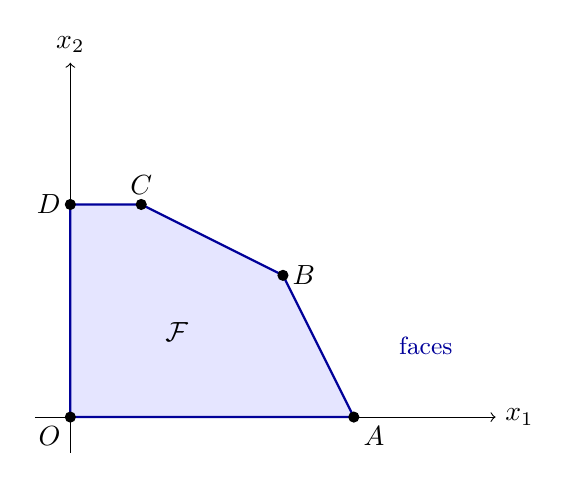
\begin{tikzpicture}[scale=0.9]
  \draw[->] (-0.5,0) -- (6,0) node[right] {$x_1$};
  \draw[->] (0,-0.5) -- (0,5) node[above] {$x_2$};
  % Poly\`edre
  \fill[blue!10] (0,0) -- (4,0) -- (3,2) -- (1,3) -- (0,3) -- cycle;
  \draw[thick, blue!60!black] (0,0) -- (4,0) -- (3,2) -- (1,3) -- (0,3) -- cycle;
  % Sommets
  \foreach \point/\name/\posi in
    {(0,0)/O/below left, (4,0)/A/below right,
     (3,2)/B/right, (1,3)/C/above, (0,3)/D/left}
    \filldraw \point circle (2pt) node[\posi] {$\name$};
  \node at (1.5,1.2) {$\mathcal{F}$};
  % Ar\^etes = faces
  \node[blue!60!black, right] at (4.5,1) {\small faces};
\end{tikzpicture}
\end{center}

\subsection{Sommets et solutions de base r\'ealisables}

\begin{definition}[Sommet]
Un point $\mathbf{v} \in P$ est un \textbf{sommet} (ou \textbf{point
extr\^emal}) du poly\`edre $P$ s'il n'existe pas deux points distincts
$\mathbf{x}, \mathbf{y} \in P$ tels que
$\mathbf{v} = \frac{1}{2}(\mathbf{x} + \mathbf{y})$.
\end{definition}

\begin{definition}[Solution de base r\'ealisable (SBR)]
Consid\'erons le syst\`eme $A\mathbf{x} = \mathbf{b}$ avec
$A \in \R^{m \times n}$, $m \le n$, $\text{rang}(A) = m$.  On partitionne
les colonnes en $B$ (base, $m$ colonnes lin\'eairement ind\'ependantes) et
$N$ (hors-base)~:
\[
  \mathbf{x}_B = B^{-1}\mathbf{b}, \qquad \mathbf{x}_N = \mathbf{0}
\]
Si $\mathbf{x}_B \ge \mathbf{0}$, alors $\mathbf{x}$ est une
\textbf{solution de base r\'ealisable}.
\end{definition}

\begin{theoreme}[\'Equivalence sommet--SBR]
\label{thm:sommet_sbr}
Soit $P = \{\mathbf{x} : A\mathbf{x} = \mathbf{b},\; \mathbf{x} \ge 0\}$
un poly\`edre.  Les assertions suivantes sont \'equivalentes~:
\begin{enumerate}
  \item $\mathbf{v}$ est un sommet de $P$.
  \item $\mathbf{v}$ est une solution de base r\'ealisable.
  \item Les colonnes de $A$ correspondant aux composantes strictement
        positives de $\mathbf{v}$ sont lin\'eairement ind\'ependantes.
\end{enumerate}
\end{theoreme}

\section{Th\'eor\`eme fondamental de la programmation lin\'eaire}

\begin{theoreme}[Th\'eor\`eme fondamental de la PL]
\label{thm:fondamental_pl}
Consid\'erons le programme lin\'eaire $\min\{\mathbf{c}^\top\mathbf{x} :
A\mathbf{x} = \mathbf{b},\; \mathbf{x} \ge 0\}$.
\begin{enumerate}
  \item Si l'ensemble r\'ealisable est non vide, il poss\`ede au moins un
        sommet.
  \item Si le probl\`eme admet une solution optimale finie, alors il existe une
        solution optimale qui est un sommet de l'ensemble r\'ealisable.
  \item Le nombre de sommets est fini (au plus $\binom{n}{m}$).
\end{enumerate}
\end{theoreme}

\begin{intuition}[title=\textbf{Pourquoi l'optimum est en un sommet~?}]
Les lignes de niveau de $\mathbf{c}^\top\mathbf{x}$ sont des hyperplans
parall\`eles.  On d\'eplace ces hyperplans dans la direction $-\mathbf{c}$
(minimisation) jusqu'\`a toucher le poly\`edre.  Le dernier point de contact
est n\'ecessairement un sommet (ou une face contenant des sommets).
\end{intuition}

\section{Exemples de formulation}

\begin{exemple}[Probl\`eme de planification de production]
Une entreprise produit $n$ articles sur $m$ machines pendant $T$ p\'eriodes.
Soit $x_{it}$ la quantit\'e de l'article $i$ produite \`a la p\'eriode $t$, et
$s_{it}$ le stock en fin de p\'eriode.

\[
\begin{aligned}
  \min \quad & \sum_{i=1}^{n}\sum_{t=1}^{T}
    (c_{it} x_{it} + h_{it} s_{it}) \\
  \text{s.c.} \quad
    & s_{i,t-1} + x_{it} - s_{it} = d_{it}
      & \forall\, i,t & \quad \text{(conservation)} \\
    & \sum_{i=1}^{n} a_{ij} x_{it} \le C_{jt}
      & \forall\, j,t & \quad \text{(capacit\'e machine $j$)} \\
    & x_{it}, s_{it} \ge 0 & \forall\, i,t
\end{aligned}
\]
o\`u $c_{it}$ est le co\^ut unitaire de production, $h_{it}$ le co\^ut de
stockage, $d_{it}$ la demande, $a_{ij}$ le temps machine unitaire.
\end{exemple}

\begin{exemple}[Probl\`eme de r\'egime alimentaire (revisit\'e)]
\label{ex:regime}
Avec les donn\'ees du chapitre pr\'ec\'edent, on formule~:
\[
\begin{aligned}
  \min \quad & 0.30 x_1 + 0.15 x_2 + 1.20 x_3 + 0.40 x_4 \\
  \text{s.c.} \quad
    & 265 x_1 + 65 x_2 + 350 x_3 + 52 x_4 \ge 2000 \\
    & 9 x_1 + 3.5 x_2 + 25 x_3 + 0.3 x_4 \ge 55 \\
    & 15 x_1 + 120 x_2 + 700 x_3 + 6 x_4 \ge 800 \\
    & x_1, x_2, x_3, x_4 \ge 0
\end{aligned}
\]
(les $x_i$ sont en hectogrammes, soit 100\,g).
\end{exemple}

\section{R\'esolution graphique d\'etaill\'ee}

\begin{exemple}[R\'esolution graphique compl\`ete]
R\'esoudre~:
\[
\begin{aligned}
  \max \quad & z = 2x_1 + 3x_2 \\
  \text{s.c.} \quad
    & x_1 + 2x_2 \le 8 \\
    & 3x_1 + 2x_2 \le 12 \\
    & x_1, x_2 \ge 0
\end{aligned}
\]

\textbf{\'Etape 1}~: Tracer les droites de contraintes.
\begin{center}
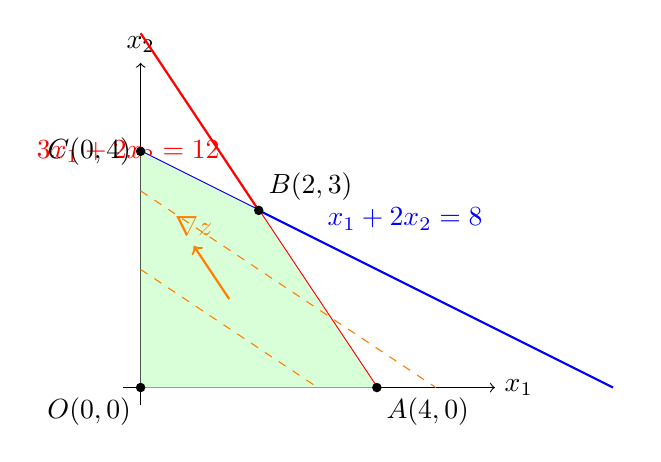
\begin{tikzpicture}[scale=0.75]
  \draw[->] (-0.3,0) -- (6,0) node[right] {$x_1$};
  \draw[->] (0,-0.3) -- (0,5.5) node[above] {$x_2$};
  % Contraintes
  \draw[thick, blue] (0,4) -- (8,0) node[right] {};
  \node[blue, above right] at (3,2.5) {$x_1+2x_2=8$};
  \draw[thick, red] (0,6) -- (4,0) node[below] {};
  \node[red, left] at (1.5,4) {$3x_1+2x_2=12$};
  % Zone réalisable
  \fill[green!15] (0,0) -- (4,0) -- (2,3) -- (0,4) -- cycle;
  % Sommets
  \filldraw (0,0) circle (2pt) node[below left] {$O(0,0)$};
  \filldraw (4,0) circle (2pt) node[below right] {$A(4,0)$};
  \filldraw (2,3) circle (2pt) node[above right] {$B(2,3)$};
  \filldraw (0,4) circle (2pt) node[left] {$C(0,4)$};
  % Lignes de niveau
  \draw[dashed, orange] (0,2) -- (3,0);
  \draw[dashed, orange] (0,3.33) -- (5,0);
  \draw[->, orange, thick] (1.5,1.5) -- (0.9,2.4) node[above] {$\nabla z$};
\end{tikzpicture}
\end{center}

\textbf{\'Etape 2}~: \'Evaluer $z$ aux sommets.
\begin{center}
\begin{tabular}{lc}
  \toprule
  Sommet & $z = 2x_1 + 3x_2$ \\
  \midrule
  $O(0,0)$ & 0 \\
  $A(4,0)$ & 8 \\
  $B(2,3)$ & \textbf{13} \\
  $C(0,4)$ & 12 \\
  \bottomrule
\end{tabular}
\end{center}

L'optimum est $z^* = 13$ atteint en $B = (2, 3)$.
\end{exemple}

\section{Cas particuliers}

\begin{definition}[Probl\`eme non r\'ealisable]
Un PL est \textbf{non r\'ealisable} (\textit{infeasible}) si $\mathcal{F}
= \emptyset$.
\end{definition}

\begin{exemple}[Non r\'ealisabilit\'e]
\[
  x_1 + x_2 \le 2, \qquad x_1 + x_2 \ge 5, \qquad x_1, x_2 \ge 0
\]
Les deux premi\`eres contraintes sont contradictoires.
\end{exemple}

\begin{definition}[Probl\`eme non born\'e]
Un PL est \textbf{non born\'e} si $z \to +\infty$ (max) ou $z \to -\infty$
(min) sur $\mathcal{F}$.
\end{definition}

\begin{definition}[Solutions optimales multiples]
Il y a \textbf{solutions optimales multiples} lorsqu'une ar\^ete enti\`ere du
poly\`edre est optimale (le gradient est parall\`ele \`a une face).
\end{definition}

\begin{definition}[D\'eg\'en\'erescence]
Une SBR est \textbf{d\'eg\'en\'er\'ee} si au moins une variable de base est nulle.
Cela arrive quand plus de $n$ contraintes sont actives en un sommet.
\end{definition}

\section{Impl\'ementation Python}

\begin{codeblock}[title=\textbf{Visualisation de la r\'egion r\'ealisable}]
\begin{minted}{python}
import numpy as np
import matplotlib.pyplot as plt
from scipy.optimize import linprog

# Résolution
c = [-2, -3]
A_ub = [[1, 2], [3, 2]]
b_ub = [8, 12]
res = linprog(c, A_ub=A_ub, b_ub=b_ub,
              bounds=[(0, None), (0, None)], method='highs')
print(f"Optimum : z = {-res.fun:.1f} en x = {res.x}")

# Tracé
fig, ax = plt.subplots(figsize=(6, 5))
x1 = np.linspace(0, 5, 300)

# Contraintes
ax.plot(x1, (8 - x1)/2, 'b-', label=r'$x_1+2x_2=8$')
ax.plot(x1, (12 - 3*x1)/2, 'r-', label=r'$3x_1+2x_2=12$')
ax.fill([0, 4, 2, 0], [0, 0, 3, 4], alpha=0.2, color='green')

ax.set_xlim(-0.5, 5.5)
ax.set_ylim(-0.5, 5.5)
ax.set_xlabel(r'$x_1$')
ax.set_ylabel(r'$x_2$')
ax.legend()
ax.set_title('Région réalisable')
plt.tight_layout()
plt.savefig('region_realisable.pdf')
\end{minted}
\end{codeblock}

\begin{codeoutput}
Optimum : z = 13.0 en x = [2. 3.]
\end{codeoutput}

\section{Exercices}

\begin{exercice}[$\star$ -- Mise sous forme standard]
Mettre sous forme standard le PL suivant~:
\[
\begin{aligned}
  \max \quad & 4x_1 - 2x_2 + 7x_3 \\
  \text{s.c.} \quad
    & x_1 + x_2 + x_3 \le 20 \\
    & 2x_1 - x_2 + 3x_3 \ge 10 \\
    & x_1 \ge 0,\; x_2 \ge 0,\; x_3 \text{ libre}
\end{aligned}
\]
\end{exercice}

\begin{exercice}[$\star$ -- R\'esolution graphique]
R\'esoudre graphiquement et identifier tous les sommets~:
\[
\begin{aligned}
  \max \quad & z = x_1 + 2x_2 \\
  \text{s.c.} \quad
    & x_1 + x_2 \le 5 \\
    & 2x_1 + x_2 \le 8 \\
    & x_2 \le 3 \\
    & x_1, x_2 \ge 0
\end{aligned}
\]
\end{exercice}

\begin{exercice}[$\star\star$ -- Poly\`edre vide ou non born\'e]
Pour chacun des PL suivants, d\'eterminer s'il est non r\'ealisable, non born\'e,
ou s'il admet une solution optimale finie~:
\begin{enumerate}
  \item $\min x_1 - x_2$ s.c.\ $x_1 + x_2 \ge 1$, $x_1, x_2 \ge 0$.
  \item $\max 2x_1 + x_2$ s.c.\ $x_1 - x_2 \le 1$, $x_1, x_2 \ge 0$.
  \item $\min x_1$ s.c.\ $x_1 + x_2 \le 4$, $x_1 - x_2 \le 2$,
        $-x_1 + x_2 \le 2$, $x_1, x_2 \ge 0$.
\end{enumerate}
\end{exercice}

\begin{exercice}[$\star\star$ -- Formulation compl\`ete]
Une raffinerie transforme du p\'etrole brut en trois produits~: essence,
diesel et k\'eros\`ene.  Deux types de brut ($B_1$ et $B_2$) sont disponibles.
Le tableau suivant donne les rendements (en \%) et les co\^uts~:

\begin{center}
\begin{tabular}{lccc|c}
  \toprule
  & Essence & Diesel & K\'eros\`ene & Co\^ut (EUR/baril) \\
  \midrule
  $B_1$ & 40\% & 35\% & 25\% & 50 \\
  $B_2$ & 30\% & 45\% & 25\% & 60 \\
  \midrule
  Demande min. (barils) & 3000 & 2000 & 1500 & \\
  \bottomrule
\end{tabular}
\end{center}

Formuler le PL minimisant le co\^ut total d'achat du brut.
\end{exercice}

\begin{exercice}[$\star\star\star$ -- D\'emonstration]
D\'emontrer que l'intersection de deux ensembles convexes est convexe.
En d\'eduire que tout poly\`edre est convexe.
\end{exercice}
